\documentclass[runningheads]{llncs}

\usepackage[T1]{fontenc}

\usepackage{graphicx}

\begin{document}

\title{Attention Is All You Need: A Position Paper}

\author{Muhammad Usman ALTAF\inst{1}\orcidID{0000-1111-2222-3333}}
%
\authorrunning{Muhammad Usman ALTAF}
%
\institute{Côte d'Azur University - SophiaTech Campus (Lucioles) 06410 Biot, France
\email{muhammad.altaf@etu.unice.fr}\\
}
%
\maketitle              
%
\begin{abstract}
The Transformer model, introduced in the groundbreaking research work \textit{Attention Is All You Need}, has revolutionized the field of Natural Language Processing (NLP). This paper evaluates the model’s contributions, focusing on its self-attention mechanism, scalability, and applications in sequence transduction tasks. This paper argues that the techniques applied make the parallelizability and performance of the model, a breakthrough in neural architecture design. This position paper provides a critical review of the model, highlighting both its innovations and areas for further research. This paper also offers comparative results from subsequent studies and proposes future directions for enhancing its capabilities.

\keywords{Transformer \and Self-Attention \and Sequence Transduction \and Natural Language Processing.}
\end{abstract}
%
%
%
\section{Introduction}
Sequence transduction, which is used in tasks like Machine Translation, Transliteration, Text-to-Speech, Spelling Correction, Speech Recognition, and Language modeling, has been dominated by recurrent neural networks (RNNs) and convolutional neural networks (CNNs). These architectures, are very effective, however, have been limited by their sequential nature, which prevents parallelization.
The inability to parallelize becomes a significant issue in sequence-to-sequence modeling because it introduces vanishing or exploding which ultimately makes it difficult to learn long-term dependencies in longer sequences.
In order to address this issue of "lost long-term dependencies", LSTMs were introduced, which made the models better at capturing long-term dependencies, yet they did not solve the problem of parallelization.
The Transformer model, proposed in the paper "Attention Is All You Need" \cite{vaswani2017attention}, replaces recurrence and convolution entirely with \textit{\textbf{self-attention mechanisms}}. This allows the model to be significantly more parallelizable and scalable, setting new benchmarks in sequence transduction modeling.

This paper evaluates the key contributions of the Transformer model, including its architectural simplicity, self-attention mechanism, and computational efficiency. It also discusses the subsequent research inspired by this work and outlines areas where further improvements can be made.


\section{Model Architecture and Innovations}
The Transformer model introduces a fully attention-based architecture, as shown in Figure \ref{fig:transformer_architecture}. The model is composed of an encoder-decoder structure, where each layer consists of multi-head self-attention and position-wise fully connected feed-forward networks.

\begin{figure}
    \centering
    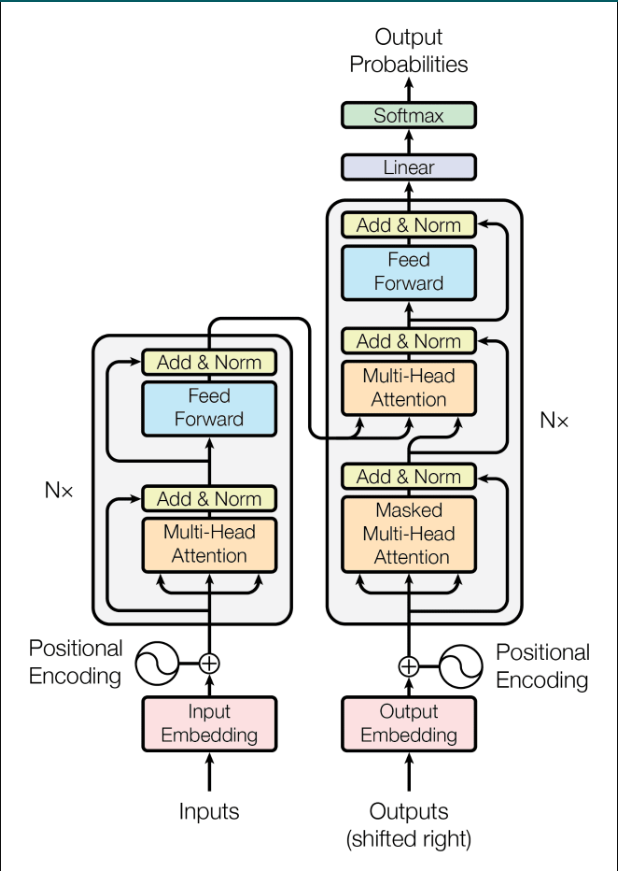
\includegraphics[width=0.7\textwidth]{transformer_Archi.png}
    \caption{The Transformer Model Architecture (Adapted from \cite{vaswani2017attention})}
    \label{fig:transformer_architecture}
\end{figure}

The breakthrough in transformers is their self-attention mechanism, which allows the model to understand global connections between inputs and outputs, unlike the RNNs which process words one by one in an order. This is achieved through the scaled dot-product attention function, which operates in parallel across all positions in the sequence.

\subsection{Self-Attention and Parallelism}
Self-attention mechanisms allow the model to draw connections from all tokens in the input sequence simultaneously, avoiding the sequential nature of RNNs and CNNs. 
The self-attention function can mathematically be written as:

\[
\text{Attention}(Q, K, V) = \text{softmax} \left( \frac{QK^T}{\sqrt{d_k}} \right)V
\]

where $Q$, $K$, and $V$ are the query, key, and value matrices, and $d_k$ is the dimension of the keys.

This mechanism not only reduces the number of sequential operations required but also improves computational efficiency, as shown in Table \ref{tab:complexity}.



\begin{table}
    \centering
    \caption{Comparison of Layer Complexity and Path Lengths (Adapted from \cite{vaswani2017attention})}
    \label{tab:complexity}
    \begin{tabular}{lccc}
    \toprule
    Layer Type & Complexity per Layer & Sequential Operations & Max Path Length \\
    \midrule
    Self-Attention & $O(n^2 \cdot d)$ & $O(1)$ & $O(1)$ \\
    Recurrent & $O(n \cdot d^2)$ & $O(n)$ & $O(n)$ \\
    Convolutional & $O(k \cdot n \cdot d^2)$ & $O(1)$ & $O(\log_k(n))$ \\
    \bottomrule
    \end{tabular}
\end{table}

\section{Advantages and Applications}
The Transformer model's ability to parallelize operations makes it ideal for large-scale tasks such as machine translation. The authors demonstrate this with their results on the WMT 2014 English-to-German and English-to-French translation tasks, where the Transformer outperforms all previous state-of-the-art models in both BLEU score and training time efficiency \cite{vaswani2017attention}.
In machine translation, the Transformer establishes new benchmarks for both quality and speed.
The improvements, along with faster training times, make the model a game-changer, especially in NLP.

\subsection{Innovations Beyond Traditional NLP}
With time, it has been observed that the Transformer model's architecture has also been extended to other domains, other than NLP. It has made some significant impacts on computer vision and speech processing too. Recent works like Vision Transformers (ViTs) \cite{dosovitskiy2020image} have demonstrated that self-attention can replace convolutions in image recognition tasks as well. This has transformed the whole paradigm of neural networks.

\section{Limitations and Challenges}
Although the Transformer model has demonstrated significant advantages over traditional recurrent and convolutional models, it still has some limitations. These include high computational costs due to its quadratic complexity in the length of the input sequence and difficulties in handling extremely long sequences.

Several efforts have been made to solve this issue. For example, models like the Reformer \cite{kitaev2020reformer} and Linformer \cite{wang2020linformer} were presented to reduce the quadratic complexity of self-attention through techniques such as locality-sensitive hashing and low-rank approximations. However, these methods also presented some trade-offs in terms of accuracy and model complexity.

Furthermore, the model's reliance on positional encodings might not be sufficient for tasks that require understanding fine-grained temporal relationships over extended periods, such as in time-series forecasting or video-based tasks. Recent developments like Relative Positional Encodings \cite{shaw2018self} and Sparse Attention mechanisms have aimed to improve the Transformer's ability to capture these relationships more effectively.

\section{Future Work and Conclusion}
Although the Transformers have been very successful, it still faces some challenges, especially when it comes to efficiently handling very long sequences. More research could be done to improve the attention mechanism to make it better at handling long sequences. Some ideas presented are to try combining the Transformer with other types of models, like those that use convolutional or recurrent layers. There's also a lot of potential for using the Transformer model for tasks outside of natural language processing (NLP).

However, the Transformer model is a big step forward in how neural networks are designed, especially for tasks where we need to convert one sequence into another. Its use of attention, instead of relying on recurrence or convolution, allows it to work more efficiently and handle larger tasks in parallel. As research continues, we expect to see this model being applied to many new areas.


\bibliographystyle{splncs04}
\bibliography{references}

\end{document}